% Author: Jan Schaumann <jschauma@netmeister.org>
% $Id: slides.tex,v 1.5 2006/04/10 14:22:04 jschauma Exp $
\special{! TeXDict begin /landplus90{true}store end }

\documentclass[xga]{xdvislides}
\usepackage[landscape]{geometry}
\usepackage{graphics}
\usepackage{graphicx}
\usepackage{colordvi}
\usepackage{multirow}

\begin{document}
\setfontphv

%%% Headers and footers
\lhead{\slidetitle}                               % default:\lhead{\slidetitle}
\chead{CS615 - Aspects of System Administration}% default:\chead{\relax}
\rhead{Slide \thepage}                       % default:\rhead{\sectiontitle}
\lfoot{\Gray{SSL, SSH}}% default:\lfoot{\slideauthor}
\cfoot{\relax}                               % default:\cfoot{\relax}
\rfoot{\Gray{\today}}

\vspace*{\fill}
\begin{center}
	\Hugesize
		CS615 - Aspects of System Administration\\ [1em]
		SSL, SSH\\ [1em]
	\hspace*{5mm}\blueline\\ [1em]
	\Normalsize
		Department of Computer Science\\
		Stevens Institute of Technology\\
		Jan Schaumann\\
		\verb+jschauma@stevens.edu+\\
		\verb+http://www.cs.stevens.edu/~jschauma/615/+
\end{center}
\vspace*{\fill}

\subsection{HW4}

\vspace*{\fill}
\begin{center}
	\Hugesize
	Anything that can go wrong will go wrong. \\
	\Normalsize
	(Error handling!)
\end{center}
\vspace*{\fill}

\subsection{HW4}
Look Ma, no temporary files!
\\

But if you must...
\begin{itemize}
	\item use {\tt mktemp(3)}
	\item {\em always} remove all temporary files
	\item don't assume you can write to the current working directory
\end{itemize}

\subsection{HW4}

\vspace*{\fill}
\Hugesize
1. Sanity Checks \\

2. ??? \\

3. Profit \\
\Normalsize
\vspace*{\fill}

\subsection{HW4}
\begin{center}
	
\includegraphics[scale=0.8]{pics/exit.eps} \\
\end{center}

\newpage
\vspace*{\fill}
\begin{center}
	\Hugesize
		SSL / TLS\\ [1em]
	\hspace*{5mm}
	\blueline\\
	\hspace*{5mm}\\
		Secure Socket Layer / Transport Layer Security
\end{center}
\vspace*{\fill}


\subsection{SSL/TLS}
Use of X.509:
\begin{itemize}
	\item public key certificates
	\item certificate revocation lists (CRLs)
	\item certificate path validation under a Public Key Infrastructure (PKI)
\end{itemize}

\subsection{SSL/TLS}
\begin{center}
	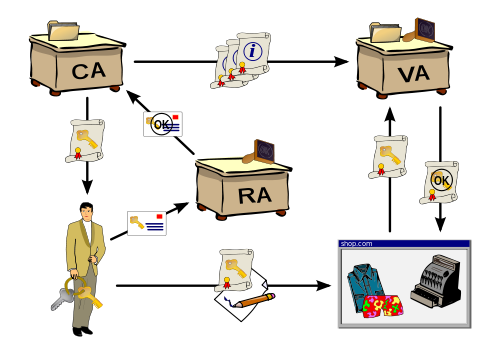
\includegraphics[scale=0.8]{pics/pki.eps} \\
CA = Certificate Authority;  RA = Registration Authority; \\
VA = Validation Authority
\end{center}

\subsection{SSL/TLS}
1. User / Company generates a {\em Certificate Signing Request} (CSR),
containing:

\begin{itemize}
	\item identifying information (distinguished name etc.)
	\item signature of data by private key
	\item chosen public key
\end{itemize}


\subsection{SSL/TLS}
1. User / Company generates a {\em Certificate Signing Request} (CSR),
containing:

\begin{itemize}
	\item identifying information (distinguished name etc.)
	\item signature of data by private key
	\item chosen public key
\end{itemize}

{\tt openssl req -new -newkey rsa:1024 -nodes \
  -keyout mykey.pem -out myreq.pem}

\subsection{SSL/TLS}
1. User / Company generates a {\em Certificate Signing Request} (CSR) \\

2. CSR submitted to Certificate Authority (CA) \\

\subsection{SSL/TLS}
1. User / Company generates a {\em Certificate Signing Request} (CSR) \\

2. CSR submitted to Certificate Authority (CA) \\

3. CA verifies information \\

\subsection{SSL/TLS}
1. User / Company generates a {\em Certificate Signing Request} (CSR) \\

2. CSR submitted to Certificate Authority (CA) \\

3. CA verifies information \\

4. CA returns certificate signed with its private key \\

\subsection{SSL/TLS}
1. User / Company generates a {\em Certificate Signing Request} (CSR) \\

2. CSR submitted to Certificate Authority (CA) \\

3. CA verifies information \\

4. CA returns certificate signed with its private key \\

5. clients can verify signatures against trusted {\em root CAs} \\


\subsection{SSL/TLS}
Some sites:

\begin{itemize}
	\item {\tt https://twitter.com}
	\item {\tt https://www.stevens.edu}
	\item {\tt https://www.google.com}
\end{itemize}

\subsection{SSL/TLS}
\vspace*{\fill}
\begin{center}
	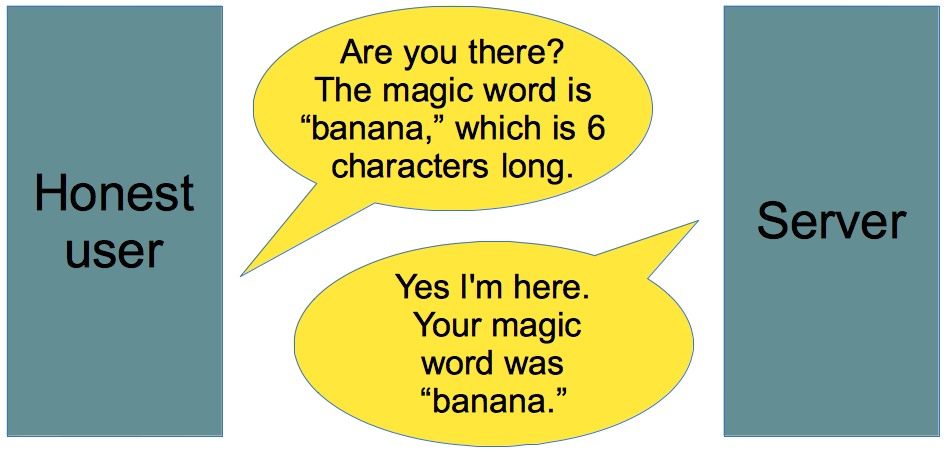
\includegraphics[scale=0.5]{pics/heartbleed1.eps} \\
\end{center}
\vspace*{\fill}

\subsection{SSL/TLS}
\vspace*{\fill}
\begin{center}
	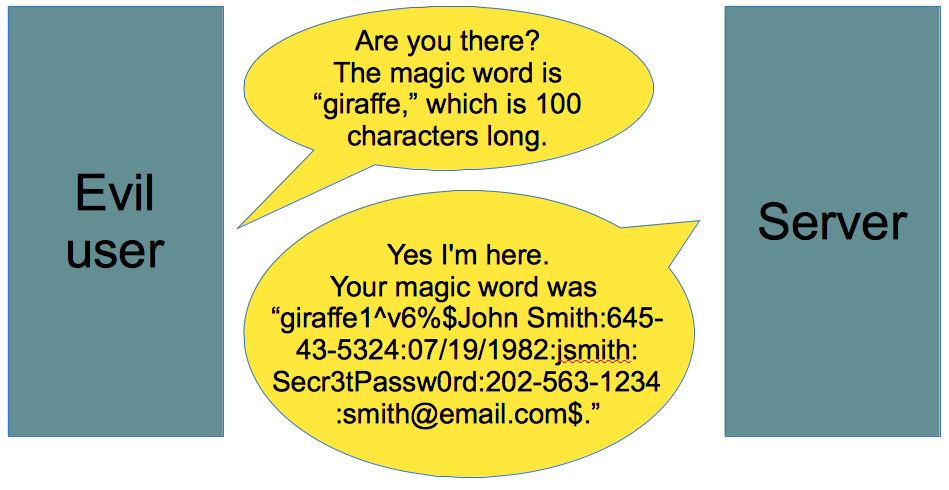
\includegraphics[scale=0.5]{pics/heartbleed2.eps} \\
\end{center}
\vspace*{\fill}

\subsection{SSL/TLS}
If you challenge the internet... \\

April 11, 2014 04:27AM -- "Can You Get Private SSL Keys Using Heartbleed?"
(We think not.) \\
{\tt http://is.gd/yMLEU5} \\

\subsection{SSL/TLS}
If you challenge the internet... \\

April 11, 2014 04:27AM -- "Can You Get Private SSL Keys Using Heartbleed?"
(We think not.) \\
{\tt http://is.gd/yMLEU5} \\

April 11, 2014 16:22PM -- "Uhm. Yeah, you can." \\
{\tt http://is.gd/6RY8oN}


\subsection{SSL/TLS}
Setting up a Man in the Middle attack site: \\

1. start instance \\

2. {\tt openssl req -x509 -nodes -days 365 -newkey rsa:1024 \
        -keyout mycert.pem -out mycert.pem} \\

3. {\tt sudo openssl s\_server -WWW -accept 443 -cert mycert.pem} \\

4. {\tt curl https://www.stevens.edu/sit/ > index.html} \\

4. go to {\tt https://<instance>:4433/index.html} \\

\subsection{SSL/TLS}

Pitfalls with PKI / CA approach: \\
{\tt https://bugzilla.mozilla.org/show\_bug.cgi?id=647959} \\

\begin{center}
	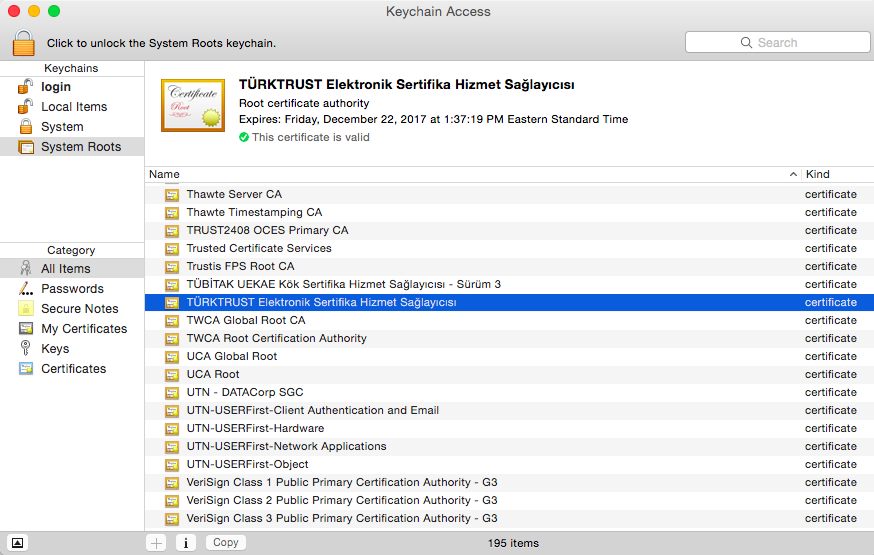
\includegraphics[scale=0.4]{pics/roots.eps} \\
	222 root CAs on this laptop...
\end{center}



%https://chamibuddhika.wordpress.com/2012/03/21/ssh-tunnelling-explained/

\newpage
\vspace*{\fill}
\begin{center}
	\Hugesize
		SSH\\ [1em]
	\hspace*{5mm}
	\blueline\\
	\hspace*{5mm}\\
		secure encrypted terminal sessions
\end{center}
\vspace*{\fill}

\subsection{SSH}
\vspace{.5in}
\begin{center}
	\Huge
	``secure'' replacement for \verb+telnet+, \verb+rlogin+, \verb+rsh+
\end{center}
\Normalsize

\subsection{SSH}
Components:
\begin{itemize}
	\item \verb+sshd(8)+
	\item \verb+ssh(1)+
\end{itemize}

\subsection{SSH}
Components:
\begin{itemize}
	\item \verb+sshd(8)+
	\item \verb+ssh(1)+
	\item \verb+scp(1)+
	\item \verb+sftp(1)+
	\item \verb+ssh-agent(1)+
	\item \verb+ssh-keygen(1)+
\end{itemize}

\subsection{SSH}
Authentication done in primarily two modes:
\begin{itemize}
	\item password authentication
	\item public-key authentication
\end{itemize}

\subsection{SSH}
Authentication done in primarily two modes:
\begin{itemize}
	\item password authentication
	\item public-key authentication
\end{itemize}
\vspace{.2in}
Communication {\em always} envolves public-key encryption.

\subsection{SSH}
Authentication done in primarily two modes:
\begin{itemize}
	\item password authentication
	\item public-key authentication
\end{itemize}
\vspace{.2in}
Communication {\em always} envolves public-key encryption.
\\

Except when it doesn't (\verb+cipher:none+).

\subsection{SSH}
SSH {\em hostkeys}
\begin{itemize}
	\item each host has (at least) one private key
	\item upon connection, it is verified against a public key
	\item discrepancies are reported (and should be investigated!)
	\item server and client perform a challenge-response handshake involving a
		random number (which becomes the session key) in SSHv1 or via
		Diffie-Hellman key agreement in SSHv2
\end{itemize}

\subsection{SSH}
SSH {\em userkeys}
\begin{itemize}
	\item used during {\em public-key authentication}
	\item the user has a {\em private} key
	\item the remote host has the corresponding {\em public} key
	\item the private key may be passphrase-protected
	\item the passphrase used and the private key itself never leave the
	      local host
\end{itemize}

\subsection{SSH}
SSH {\em agents}:
\begin{itemize}
	\item allow the user to add multiple keys once, then no longer need to
		provide the passphrases
	\item agents can be {\em forwarded}
	\item communication happens through a unix-domain socket
\end{itemize}

\subsection{SSH}
...and then there are tunnels...
\begin{center}
	
\includegraphics[scale=1.8]{pics/tunnel.eps} \\
\end{center}


\subsection{SSH configuration}
\vspace{.5in}
\begin{center}
	\Huge
	\verb+sshd_config(5)+
	\\
	\verb+ssh_config(5)+
\end{center}
\Normalsize

\subsection{Reading}
SSL/TLS
\begin{itemize}
	\item {\tt http://www.madboa.com/geek/openssl/}
	\item {\tt https://www.imperialviolet.org/2014/04/19/revchecking.html}
	\item {\tt http://www.vox.com/cards/heartbleed/what-is-the-heartbleed-bug}
\end{itemize}

SSH:
\begin{itemize}
	\item \verb+ssh(1)+
	\item \verb+ssh_config(5)+
	\item \verb+sshd_config(5)+
	\item \verb+sshd(8)+
	\item RFC4255 -- SSHFP in DNS
\end{itemize}


\end{document}
